% UG 1399 document
% Chapter I

\section{Design Principles for Software Programmers}

\subsection{Introduction}
The discussion in this section is tool-agnostic and the concepts introduced are common to most HLS tools. 

\begin{itemize}
  \item \textbf{Throughput} is defined as the number of specific actions executed per unit of time or results produced per unit of time.
  \item \textbf{Performance} is defined as higher throughput with low
  power consumption. Lower power consumption is just as important as higher throughput.
  
\end{itemize}


\subsection{Computer Architecture}

The von Neumann architecture is the basis of almost all computing done today even though it was designed more than 7 decades ago. This architecture was deemed optimal for a large class of
applications and has tended to be very flexible and programmable. 
However, as application demands started to stress the system, CPUs began supporting the execution of multiple
processes. Multithreading and/or Multiprocessing can include multiple system processes (\eg executing two or more programs at the same time), or it can consist of one process that
has multiple threads within it. Multi-threaded programming using a shared memory system
became very popular as it allowed the software developer to design applications by keeping parallelism in mind but with a fixed CPU architecture. 

\par But when multi-threading and the ever-increasing CPU speeds could no longer handle the data processing rates, multiple CPU cores and hyperthreading were used to improve throughput as shown in the figure on the right.

\begin{highlight}
  This general purpose flexibility comes at a cost in terms of power and peak throughput.  
\end{highlight}

To achieve higher throughput, the workload must be closer
to memory, and/or into specialized functional units. So the new challenge is to design a new programmable architecture in such a way that you can maintain just enough programmability while achieving higher performance and lower power costs.

\par A field-programmable gate array (FPGA) provides for this kind of programmability and offers enough memory bandwidth to make this a high-performance and lower power cost solution. Unlike a CPU that executes a program, an FPGA can be configured into a custom hardware circuit that will respond to inputs in the same way that a dedicated piece of hardware would behave.

\par Reconfigurable devices such as FPGAs contain computing elements of extremely flexible granularities, ranging from elementary logic gates to complete arithmetic-logic units such as DSP blocks. At higher granularities, user-specified composable units of logic called kernels can then be strategically placed on the FPGA device to perform various roles. This characteristic of reconfigurable FPGA devices allows the creation of custom macro-architectures and gives FPGAs a big advantage over traditional CPUs/GPUs in utilizing application-specific parallelism. Computation can be spatially mapped to the device, enabling much higher operational throughput than processor-centric platforms. Today's latest FPGA devices can also contain processor cores (Arm-based) and other hardened IP blocks that can be used without having to program them into the programmable fabric.

\subsection{Three Paradigms for Programming FPGAs}

While FPGAs can be programmed using lower-level Hardware Description Languages (HDLs) such as Verilog or VHDL, there are now several High-Level Synthesis (HLS) tools that can take an algorithmic description written in a higher-level language like C/C++ and convert it into lower-level hardware description languages such as Verilog or VHDL. This can then be processed by downstream tools to program the FPGA device. The main benefit of this type of flow is that you
can retain the advantages of the programming language like C/C++ to write efficient code that can then be translated into hardware. 

\par A program written in C/C++ is essentially written for the von Neumann style of architecture where each instruction is executed sequentially. In order to achieve high performance, the HLS tool must infer parallelism in the sequential code and exploit it to achieve
greater performance. 

\par Many coding techniques (such as RTTI, recursion,
and dynamic memory allocation) have no direct equivalency in hardware. Hence, arbitrary, off-the-shelf software cannot be efficiently converted into hardware. At a bare minimum, such software needs
to be examined for non-synthesizable constructs and the code needs to be refactored to make it synthesizable. Even the automatically converted (or synthesized) program with acceptable quality of results (QoR), will require additional work to help the HLS tool achieve the desired performance goals. 

\subsubsection{Producer-Consumer Paradigm}
In a multithreaded program, there is usually a master
thread that performs some initialization steps and then forks off a number of child threads to do some parallel computation and when all the parallel computation is done, the main thread
collates the results and writes to the output. 

\par Similarly, in FPGAs, same fork/join type of parallelism is applied.
A key pattern for throughput on FPGAs is the producer-consumer paradigm. The producerconsumer
paradigm is applied to a sequential program and it is converted to extract functionality that can be executed in parallel to improve performance. The goal is to decompose the program in such a way
that you can identify tasks that can potentially execute in parallel and therefore increase the throughput of the system.

\par The first step is to understand the program workflow and identify the independent tasks or functions. Two independent tasks need not wait to happen sequentially instead, they can start the execution with interleaving/overlapping. This is referred as Producer-Consumer Paradigm. On FPGAs, due to the custom architecture, the producer and consumer threads can be executed simultaneously with little or no overhead leading to a considerable improvement in throughput unlike a regular CPU. 

\subsubsection{Streaming Data Paradigm "Dataflow"}
A stream is an important abstraction: it represents an unbounded, continuously updating data set, where unbounded means "of unknown or of unlimited size". A stream can be a sequence of data
(scalars or buffers) flowing unidirectionally between a source (producer) process and a destination (consumer) process. 

\par Decomposing your algorithm into producerconsumer
relationships that communicate by streaming data through the network has several advantages. 

\begin{itemize}
  \item It lets the programmer define the algorithm in a sequential manner and the parallelism is extracted through other means (such as by the compiler). 
  \item Complexities like synchronization between the tasks etc. are abstracted away.
  \item It allows the producer and the consumer tasks to process data simultaneously, which is key for achieving higher throughput.
  \item Another benefit is cleaner and simpler code.
\end{itemize}


\subsubsection{Pipelining Paradigm}
Another optimization that allows for finer-grained parallelism is pipelining. Pipelining is a process which enables parallel execution of program instructions. 

\begin{highlight}
  Pipelining does not decrease the latency, that is, the total time for one item to go through the whole system. It does however increase the system's throughput, that is, the rate at which new
  items are processed after the first one.
\end{highlight}

\begin{itemize}
  \item Delay associated with the number of clock cycles lost before the first valid output is delivered is referred to as \textit{Iteration Latency}.
  \item \textit{Initiation Interval (II)} of the pipeline is defined as the time taken by the design between delivering two consecutive outputs post Iteration Latency or first output.  
  \item The overall time taken to deliver all the outputs through iterations is referred to as the \textit{Total Latency} of the pipeline.
\end{itemize}

\begin{highlight}
  Total Latency = Iteration Latency + II * (iterations - 1)  
\end{highlight}

Pipelining is a classical micro-level architectural optimization that can be applied to multiple levels of abstraction. Similar tp task-level pipelining with the producer-consumer paradigm, pipelining applies to the instruction-level as well. This is in fact key to keeping the producer-consumer pipelines (and streams) filled and busy. The producer-consumer pipeline will only be efficient if each task produces/consumes data at a high rate, and hence the need for the
instruction-level pipelining (ILP).

\subsection{Combining the Three Paradigms}
Functions and loops are the main focus of most optimizations in the user's program. Each function can be
converted into a specific hardware component. Each such hardware component can be instantiated in
the hardware design. Each hardware component will in turn be composed of many
smaller predefined components that typically implement basic functions such as add, sub, and
multiply etc. Functions may call other functions although recursion is not supported. 

\par Functions that
are small and called less often can be also inlined into their callers just like how software
functions can be inlined. In this case, the resources needed to implement the function are
subsumed into the caller function's component which can potentially allow for better sharing of
common resources. Constructing your design as a set of communicating functions lends to inferring parallelism when executing these functions.

\begin{highlight}
  An inline function is a function for which the compiler copies the code from the function definition directly into the code of the calling function rather than creating a separate set of instructions in memory. This eliminates call-linkage overhead and can expose significant optimization opportunities.   
\end{highlight}

Loops are one of the most important constructs in your program. Since the body of a loop is
iterated over a number of times, this property can be easily exploited to achieve better
parallelism. There are several transformations (such as {\it pipelining} and {\it unrolling}) that can be made
to loops and loop nests in order to achieve efficient parallel execution. These transformations
enable both memory-system optimizations as well as mapping to multi-core and SIMD execution
resources.

\par In multiple cases, programs are expressed as operations
over large data structures with data dependencies across the
iterations of the loop. Such data dependencies impact the parallelism achievable in the loop. In many such cases, the code must be restructured such that loop iterations can be executed
efficiently and in parallel on modern parallel platforms.

\par An efficient technique to improve throughput and reuse computational resources is to pipeline operators, loops, and/or functions.

\begin{highlight}
  The three paradigms show how parallelism can be
  achieved in the design without needing the complexities of multi-threading and/or parallel programming languages. 
\end{highlight} 

\subsection{Conclusion - A Prescription for performance}
Checklist of high-level actions for achieving performance on reconfigurable FPGA platforms:

\begin{itemize}
  \item Software written for CPUs and software written for FPGAs is fundamentally different. 
  \item Right from the start of your project, establish a flow that can functionally verify the source code changes that are being made. Testing the software against a reference model or using golden vectors are common practices.
  \item (\textbf{Producer - Consumer Paradigm: })Focus first on the macro-architecture of your design.
  \item Visualize parallelism with function execution timeline and compare with the final achieved results.
  \item Only start coding or refactoring your program once you have the macro-architecture and the activity timeline established.
  \item As a general rule, the HLS compiler will only infer task-level parallelism from function calls.
  \item \textbf{Data flow: } Decompose/partition the original algorithm into smaller components that talk to each other via streams (Visualize the data flow).
  \begin{itemize}
    \item Smaller modular components have the advantage that they can be replicated when needed to improve parallelism.
    \item Avoid having communication channels with very wide bit-widths. Decomposing such wide channels into several smaller ones will help implementation on FPGA devices.
    \item Large functions (written by hand or generated by inlining smaller functions) can have nontrivial control paths that can be hard for tools to process.
    \item Smaller functions with simpler control paths will aid implementation on FPGA devices.
    \item Aim to have a single loop nest (with either fixed loop bounds that can be inferred by HLS tool, or by providing loop trip count information by hand to the HLS tool) within each function. This greatly facilitates the measurement and optimization of throughput. (Not be applicable for all designs)
    \item 
  \end{itemize}
  \item \textbf{Throughput: } Have an overall vision about what rates of processing will be required during each phase of your design is important. Knowing this will influence how you write your application for FPGAs.
  \begin{itemize}
    \item Try to locate the critical path(s) in the design a potential bottleneck.  
    \item HLS GUI tools and/or the simulation waveform viewer can be used to visualize such throughput issues.
    \item Stream-based communication allows consumers to start processing as soon as producers start producing which allows for overlapped execution (which in turn increases parallelism
    and throughput).
    \item In order to keep the producer and consumer tasks running constantly without any hiccups, optimize the execution of each task to run as fast as possible using techniques such as
    pipelining and the appropriate sizing of streams.    
  \end{itemize}
  \item Think about the granularity (and overhead) of the streaming channels with respect to synchronization. 
  \item PIPO and FIFO : The usage of PIPO channels allows you to overlap task execution without the fear of deadlock while explicit manual streaming FIFO channels allow you to start the overlapped execution sooner (than PIPOs) but require careful adjustment of FIFO sizes to avoid deadlocks.
  \item Locate and remove un-synthesizable C/C++ coding styles.
  \item Use the reports generated by the HLS compiler to guide the optimization process. 
  \item Another important aspect to consider is the interface of accelerated function or kernel. The interface of the kernel to the outside world is an important element of the eventual system design.
\end{itemize}



\clearpage
\section{Introduction to Vitis/Vivado HLS}

Vitis/Vivado HLS is a high-level synthesis tool that allows C, C++, and OpenCL functions to become hardwired onto the device logic fabric and RAM/DSP blocks. Vitis/Vivado HLS implements hardware kernels in the Vitis application acceleration development flow and uses C/C++ code for developing RTL IP for Xilinx device designs in the Vivado Design Suite.

\par In the Vitis application acceleration flow, the Vitis/Vivado HLS tool automates much of the code modifications required to implement and optimize the C/C++ code in programmable logic and to achieve low latency and high throughput. The inference of required pragmas to produce the right interface for your function arguments and to pipeline loops and functions within your code is the foundation of Vitis/Vivado HLS in the application acceleration flow. Vitis/Vivado HLS also supports customization of your code to implement different interface standards or specific optimizations to achieve your design objectives.

Following is the Vitis/Vivado HLS design flow:
\begin{enumerate}
    \item Compile, simulate, and debug the C/C++ algorithm.
    \item View reports to analyze and optimize the design.
    \item Synthesize the C algorithm into an RTL design.
    \item Verify the RTL implementation using RTL co-simulation.
    \item Package the RTL implementation into a compiled object file (.xo) extension, or export to an RTL IP.
\end{enumerate}

\subsection{High-Level Synthesis Benefits}
High-level synthesis bridges hardware and software domains, providing the following benefits:
\begin{itemize}
  \item Improved productivity for hardware designers:\\ Hardware designers can work at a higher level of abstraction while creating high-performance hardware.
  \item Improved system performance for software designers:\\ Software developers can accelerate the computationally intensive parts of their algorithms on a new compilation target, the FPGA. 
\end{itemize}

Using a high-level synthesis design methodology allows you to:
\begin{description}
  \item[Develop algorithms at the C-level] Work at a level that is abstract from the implementation details, which consume development time.
  \item[Verify at the C-level] Validate the functional correctness of the design more quickly than with traditional hardware description languages.
  \item[Control the C synthesis process through optimization directives] Create specific high-performance hardware implementations.
  \item[Create multiple implementations from the C source code using optimization directives] Explore the design space, which increases the likelihood of finding an optimal implementation.
  \item[Create readable and portable C source code] Retarget the C source into different devices as well as incorporate the C source into new projects.
\end{description}

\subsection{High-Level Synthesis Basics}   
High-level synthesis includes the following phases:
\begin{itemize}
  \item Scheduling
    Determines which operations occur during each clock cycle based on:
    \begin{itemize}
      \item Length of the clock cycle or clock frequency.
      \item Time it takes for the operation to complete, as defined by the target device.
      \item User-specified optimization directives.
      \item Operation's dependencies.
      \item Available resource allocation.
    \end{itemize}
    If the clock period is longer or a faster FPGA is targeted, more operations are completed within a single clock cycle, and all operations might complete in one clock cycle. Conversely, if the clock period is shorter or a slower FPGA is targeted, high-level synthesis automatically schedules the operations over more clock cycles, and some operations might need to be  implemented as multicycle resources.
    \item Binding
    Determines which hardware resource implements each scheduled operation. To implement
    the optimal solution, high-level synthesis uses information about the target device.
    \item Control logic extraction
    Extracts the control logic to create a finite state machine (FSM) that sequences the operations
    in the RTL design.
\end{itemize}

\clearpage
\section{Vitis/Vivado HLS Process Overview}
Vitis/Vivado HLS is project based and can contain multiple variations called "solutions" to drive synthesis
and simulation. Each solution can target either the Vivado IP flow, or the Vitis Kernel flow. Based
on the target flow, each solution will specify different constraints and optimization directives.

\par The following are the synthesis, analysis, and optimization steps in the typical design flow:
\begin{enumerate}
  \item Create a new Vitis/Vivado HLS project.
  \item Verify the source code with C simulation.
  \item Run high-level synthesis to generate RTL files.
  \item Analyze the results by examining latency, initiation interval (II), throughput, and resource utilization.
  \item Optimize and repeat as needed.
  \item Verify the results using C/RTL Co-simulation.
\end{enumerate}

Vitis/Vivado HLS implements the solution based on the target flow, default tool configuration, design
constraints, and any optimization pragmas or directives you specify. You can use optimization
directives to modify and control the implementation of the internal logic and I/O ports,
overriding the default behaviors of the tool.

\par The C/C++ code is synthesized as follows:
\begin{itemize}
  \item Top-level function arguments synthesize into RTL I/O port interfaces automatically by Vitis/Vivado HLS. 
  \item Sub-functions of the top-level C/C++ function synthesize into blocks in the hierarchy of the RTL design.
  \begin{itemize}
    \item The final RTL design includes a hierarchy of modules or entities that correspond with the original top-level C function hierarchy.
    \item Vitis/Vivado HLS automatically inlines sub-functions into higher level functions, or the top-level function as needed to improve performance.
    \item By default, each call of the C sub-function uses the same instance of the RTL module.
  \end{itemize}
  \item Loops in the C functions are kept rolled and are pipelined by default to improve performance.
  \begin{itemize}
    \item The Vitis/Vivado HLS tool will not unroll loops unless it improves the performance of the solution. 
    \item Loops can be manually unrolled.
    \item Loops can also be pipelined, either with a finite-state machine fine-grain implementation (loop pipelining) or with a more coarse-grain handshake-based implementation (dataflow).
  \end{itemize}
  \item Arrays in the code are synthesized into block RAM (BRAM), LUT RAM, or UltraRAM in the final FPGA design.
  \begin{itemize}
      \item If the array is on the top-level function interface, high-level synthesis implements the array as ports with access to a block RAM outside the design.
      \item The type of memory used can be reconfigured, or read/write memory transfers can be reconfigured.
  \end{itemize}
\end{itemize}

After synthesis, you can analyze the results in the various reports produced to determine the quality of your results. After analyzing the results, you can create additional solutions for your
project specifying different constraints and optimization directives, and synthesize and analyze
those results. You can compare results between different solutions to see what has worked and
what has not. You can repeat this process until the design has the desired performance
characteristics. Using multiple solutions allows you to proceed with development while retaining
prior solutions.


\par These are the performance metrics:
\begin{itemize}
  \item Area: Amount of hardware resources required to implement the design based on the resources
  available in the FPGA, including look-up tables (LUT), registers, block RAMs, and DSP48s.
  \item Latency: Number of clock cycles required for the function to compute all output values.
  \item Initiation interval (II): Number of clock cycles before the function can accept new input data.
  \item Loop iteration latency: Number of clock cycles it takes to complete one iteration of the loop.
  \item Loop initiation interval: Number of clock cycles before the next iteration of the loop starts to
  process data.
  \item Loop latency: Number of cycles to execute all iterations of the loop.
\end{itemize}

\clearpage
\section{Creating project with Vitis HLS}
Inputs of the Vitis/Vivado HLS are:
\begin{itemize}
  \item \textbf{C function written in C, C++11, C++14, or SystemC}\\ is the primary input to Vitis/Vivado HLS. The function can contain a hierarchy of subfunctions.
  \item \textbf{Constraints}\\ are required and include the clock period, clock uncertainty, and FPGA target. The clock uncertainty defaults to 12.5\% of the clock period if not specified.
  \item \textbf{Directives}\\ are optional and direct the synthesis process to implement a specific behavior or optimization.
  \item \textbf{C test bench and any associated files}\\ are needed to simulate the C function prior to synthesis and to verify the RTL output using C/RTL Cosimulation.
\end{itemize}

Outputs of the Vitis/Vivado HLS are:
\begin{itemize}
  \item \textbf{RTL implementation files in hardware description language (HDL) formats}\\ This is the primary output from Vitis/Vivado HLS. RTL IP produced by Vitis/Vivado HLS is available in both Verilog (IEEE 1364-2001), and VHDL (IEEE 1076-2000) standards, and can be synthesized and implemented into Xilinx devices.
  \item \textbf{Report files}\\ This output is the result of synthesis, C/RTL co-simulation, and IP packaging.
  \item \textbf{Compiled object files (.xo)(Vitis)}\\ This output lets you create compiled hardware functions for use in the Vitis application acceleration development flow. Vitis/Vivado HLS produces this output when called as part of the compilation process from the Vitis tool flow, or when invoked as a stand-alone tool in the bottom up flow.
\end{itemize}

The \figref{VitisFlow} shows an overview of the Vitis/Vivado HLS input and output files.
\begin{figure}[H]
  \begin{center}
      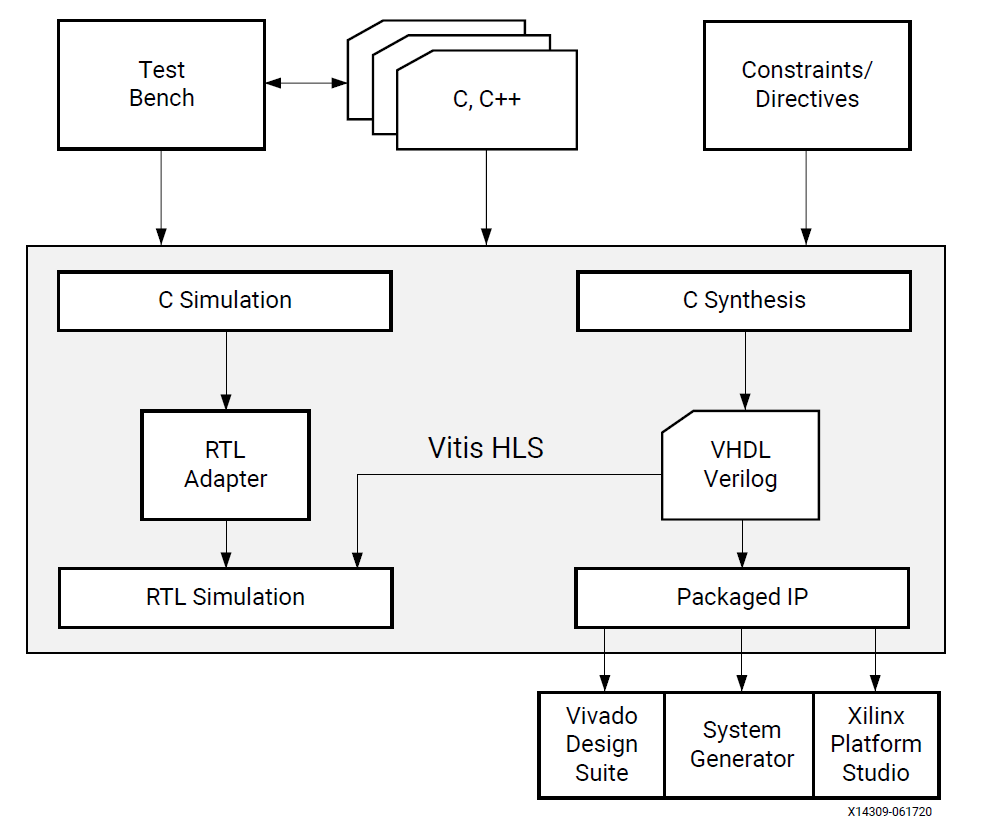
\includegraphics[width=0.7\textwidth]{images/VitisFlow.png}
      \caption{Vitis/Vivado HLS Design Flow}
      \label{VitisFlow}
  \end{center}
\end{figure}

\subsection{Coding C/C++ Functions}
\subsubsection{Coding Style}
In any C program, the top-level function is called main(). In the Vitis HLS design flow, you can specify any sub-function below main() as the top-level function for synthesis. You cannot
synthesize the top-level function main(). Following are additional rules:
\begin{itemize}
  \item Only one function is allowed as the top-level function for synthesis.
  \item Any sub-functions in the hierarchy under the top-level function for synthesis are also synthesized.
  \item If you want to synthesize functions that are not in the hierarchy under the top-level function for synthesis, you must merge the functions into a single top-level function for synthesis.
\end{itemize}

\subsubsection{C/C++ Language Support}
Vitis HLS supports the C/C++ 11/14 for compilation/simulation. 
Vivado HLS supports the following standards for C compilation/simulation: ANSI-C (GCC 4.6), C++ (G++ 4.6), SystemC (IEEE 1666-2006, version 2.2).

Vitis/Vivado HLS supports many C and C++ language constructs, and all native data types for each language, including float and double types. However, synthesis is not supported for some constructs, including:
\begin{itemize}
  \item \textbf{Dynamic memory allocation}\\  An FPGA has a fixed set of resources, and the dynamic creation and freeing of memory resources is not supported.
  \item \textbf{Operating system (OS) operations}\\  All data to and from the FPGA must be read from the input ports or written to output ports. OS operations, such as file read/write or OS queries like time and date, are not supported. Instead, the host application or test bench can perform these operations and pass the data into the function as function arguments.
\end{itemize}

\subsubsection{Libraries in Vitis HLS}
Vitis HLS provides foundational C libraries allowing common hardware design constructs and functions to be easily modeled in C and synthesized to RTL. Vitis HLS provides the following C libraries to extend the standard C languages:

\begin{itemize}
  \item Arbitrary Precision Data Types Library: Arbitrary precision data types let your C code use variables with smaller bit-widths than standard C or C++ data types, to enable improved performance and reduced area in hardware.
  \item Vitis HLS Math Library: Used to specify standard math operations for synthesis into RTL and implementation on Xilinx devices.
  \item HLS Stream Library: For modeling and compiling streaming data structures.
  \item In addition, the Vitis accelerated libraries are available for use with Vitis HLS, including common functions of math, statistics, linear algebra and DSP; and also supporting domain specific applications, like vision and image processing, quantitative finance, database, data analytics, and data compression. Documentation for the Vitis accelerated libraries can be found at \url{https://xilinx.github.io/Vitis_Libraries/}
\end{itemize}

\subsection{Specifying the Clock Frequency}
For C and C++ designs only a single clock is supported. The same clock is applied to all functions in the design. The clock period, can be set in a particular solution. Vitis HLS uses the concept of a clock uncertainty to provide a user defined timing margin. The default clock uncertainty, when it is not specified, is 27\% of the clock period.

\par Using the clock frequency and device target information Vitis HLS estimates the timing of operations in the design but it cannot know the final component placement and net routing:
these operations are performed by logic synthesis of the output RTL. As such, Vitis HLS cannot estimate the exact delays.

\par Vitis HLS aims to satisfy all constraints: timing, throughput, latency. However, if a constraints cannot be satisfied, Vitis HLS always outputs an RTL design.

\clearpage
\section{C simulation verification}
Verification in the Vitis HLS flow can be separated into two distinct processes.
\begin{enumerate}
  \item Pre-synthesis validation that the C program correctly implements the required functionality which is referred to as \textbf{C simulation}.
  \item Post-synthesis verification that the generated RTL code performs as expected which is referred to as \textbf{C/RTL co-simulation}.
\end{enumerate}

Using C to develop and validate the algorithm before synthesis is much faster than developing and debugging RTL code. Vitis HLS uses the test bench to compile and execute the C simulation. Vitis HLS also uses the same test bench to verify the RTL output of synthesis during C/RTL Co-Simulation in Vitis HLS. The first step in high-level synthesis should be to validate the C code functionality, before generating RTL code, by performing simulation using a well written test bench.
  
\subsection{Writing a Test Bench}
\begin{enumerate}
  \item A C test bench includes a main() as a top-level function, that calls the function to be synthesized by the Vitis HLS project.
  \item The test bench includes the main() function which verifies the top-level functionality for synthesis by providing stimuli and calling the function for synthesis, and by consuming and validating its output.
  \item The test bench should execute the top-level function for multiple transactions, allowing many different data values to be applied and verified. 
  \item The test bench is only as good as the variety of tests it performs. 
  \item In addition, the test bench must provide multiple transactions if II is to be calculated during RTL simulation.
  \item The test bench should ideally be \textbf{Self-checking}, and should validate the results from the function to be synthesized are correct.
  \item If the results are correct the test bench returns a value of 0 to main(). Otherwise, the test bench should return any non-zero value.
  \item The test bench can return any non-zero value. A complex test bench can return different values depending on the type of failure. If the test bench returns a non-zero value after C simulation or  C/RTL co-simulation, Vitis HLS reports an error and simulation fails.
  \item As Vitis HLS reuses the C test bench for RTL verification, it requires that the test bench and any associated files be denoted as test bench files when they are added to the Vitis HLS project.
\end{enumerate}


\clearpage
\section{C Synthesis}
During C synthesis, the C/C++ source code is synthesized into an RTL implementation.

Parameters of the C synthesis:
\begin{itemize}
  \item Latency: Number of clock cycles required for the function to compute all output values.
  \item Initiation interval (II): Number of clock cycles before the function can accept new input data.
  \item Loop iteration latency: Number of clock cycles it takes to complete one iteration of the loop.
  \item Loop iteration interval: Number of clock cycles before the next iteration of the loop starts to
  process data.
  \item Loop latency: Number of cycles to execute all iterations of the loop.
  \item Resource Utilization: Amount of hardware resources required to implement the design based on the resources available in the FPGA, including look-up tables (LUT), registers, block RAMs, and DSP blocks.
\end{itemize}

\clearpage
\section{Analyzing the Results of Synthesis}
After synthesis completes, Vitis HLS automatically creates synthesis reports to help you understand and analyze the performance of the implementation. Examples of these reports include the Synthesis Summary report, Schedule Viewer, Function Call Graph, and Dataflow Viewer.

\begin{itemize}
  \item \textbf{Schedule Viewer}: Shows each operation and control step of the function, and the clock cycle that it executes in.
  \item \textbf{Dataflow Viewer}: Shows the dataflow structure inferred by the tool, inspect the channels (FIFO/PIPO), to let you examine the effect of channel depth on performance.
  \item \textbf{Function Call Graph Viewer}: Displays your full design after C Synthesis or C/RTL Cosimulation to show the throughput of the design in terms of latency and II.
\end{itemize}

The Vitis HLS tool also provides additional views to expand on the information available for analysis of your design.

\begin{itemize}
  \item \textbf{Module Hierarchy}: Shows the resources and latency contribution for each block in the RTL hierarchy It also indicates any II or timing violations. In case of timing violations, the hierarchy
  window will also show the total negative slack observed in a specific module.
  \item \textbf{Performance Profile}: Shows details on the performance of the block currently selected in the Module Hierarchy view. Performance is measured in terms of latency and the initiation interval, and includes details on whether the block was pipelined or not.
  \item \textbf{Resource Profile}: Shows the resources used at the selected level of hierarchy, and shows the control state of the operations used.
  \item \textbf{Properties view}: Shows the properties of the currently selected control step or operation in the Schedule Viewer. 
\end{itemize}

\subsection{Schedule Viewer}
The Schedule Viewer provides a detailed view of the synthesized RTL, showing each operation and control step of the function, and the clock cycle that it executes in. It helps you to identify any loop dependencies that are preventing parallelism, timing violations, and data dependencies. The Schedule Viewer is displayed by default in the Analysis perspective.

\subsection{Function Call Graph Viewer}
The new Function Call Graph Viewer, which can be opened from the Flow Navigator, illustrates your full design after C Synthesis or C/RTL Co-simulation. The goal of this viewer is to show the throughput of the design in terms of latency and II. It helps identify the critical path in your design and helps you identify bottlenecks in the design to focus on to improve throughput. It can also show the paths through the design where throughput may be imbalanced leading to FIFO stalls and/or deadlock.

\par In some cases, the displayed hierarchy of the design might not be the same as your source code
as a result of HLS optimizations that convert loops into function pipelines, etc. Functions that are
in-lined will no longer be visible in the call graph, as they are no longer separate functions in the
synthesized code. If multiple instances of a function are created, each unique instance of the function is shown in the call graph. 

\par The call graph displays functions as rectangular boxes, and loops as oval boxes, each with II, latency, and resource or timing data depending on the specific view. Before C/RTL cosimulation is completed the performance and resource metrics that are shown in the graph are from the C Synthesis phase, and are therefore estimates from the HLS tool.

\par After co-simulation, actual II and latency numbers are reported along with stalling percentages, and this information is back annotated from data collected during co-simulation. 

\par Heat Map feature can also be used to highlight several metrics of interest:
\begin{itemize}
  \item II (min, max, avg)
  \item Latency (min, max, avg)
  \item Stalling Time Percentage
\end{itemize}

The heat map uses color coding to highlight problematic modules. Using a color scale of red to green where red indicates the high value of the metric (\ie highest II or highest latency) while green indicates a low value of the metric in question. The colors that are neither red nor green
represent the range of values that are in between the highest and lowest values. This helps in quickly identifying the modules that need attention. 


\subsection{Dataflow Viewer}
The DATAFLOW optimization is a dynamic optimization which can only be fully understood after the RTL co-simulation is complete. Due to this fact, the Dataflow viewer lets you see the dataflow structure inferred by the tool, inspect the channels (FIFO/PIPO), and examine the effect
of channel depth on performance. Performance data is back-annotated to the Dataflow viewer from the co-simulation results.

\par One must apply the DATAFLOW pragma or directive to the design for the Dataflow viewer to be populated. Dataflow can be applied to the top-level function, or specify regions of a function, or loops. The Dataflow viewer displays a representation of the dataflow graph structure, showing
the different processes and the underlying producer-consumer connections.


Features of the Dataflow viewer include the following:
\begin{itemize}
  \item Source Code browser.
  \item Automatic cross-probing from process/channel to source code.
  \item Filtering of ports and channel types.
  \item Process and Channel table details the characteristics of the design: 
  \begin{itemize}
    \item Channel Profiling (FIFO sizes etc), enabled from Solution Settings dialog box.
    \item Process Read Blocking/Write Blocking/Stalling Time reported after RTL co-simulation.
    \item Process Latency and II displayed.
    \item Channel type and widths are displayed in the Channel table.
    \item Automatic cross-probing from Process and Channel table to the Graph and Source browser.
    \item Hover over channel or process to display tooltips with design information.
  \end{itemize}
\end{itemize}

The Dataflow viewer can help with performance debugging your designs. When the design deadlocks during RTL co-simulation, the GUI will open the Dataflow viewer and highlight the channels and processes involved in the deadlock so you can determine what the cause is.


\clearpage
\section{Optimizing the HLS Project}
After analysis, designer will most likely need or want to optimize the performance of your function. Even if it is performing well there may be opportunities for improvement. One can add optimization directives directly into the source code as compiler pragmas, using various HLS PRAGMAS, or by using Tcl set\_directive commands to apply optimization directives in a Tcl script to be used by a solution. In addition to optimization pragmas and directives, Vitis HLS provides a number of configuration settings to let you manage the default results of simulation and synthesis. 

\subsection{Creating Additional Solutions}
The most typical use of Vitis HLS is to create an initial design, analyze the results, and then perform optimizations to meet the desired area and performance goals. This is often an iterative process, requiring multiple steps and multiple optimizations to achieve the desired results. Solutions offer a convenient way to configure the tool, add directives to your function to improve the results, and preserve those results to compare with other solutions.

\subsection{Adding Pragmas and Directives}
Vitis HLS pragmas and directives let you configure the synthesis results for your code.
\begin{itemize}
  \item HLS Pragmas are added to the source code to enable the optimization or change in the original source code. Every time the code is synthesized, it is implemented according to the specified pragmas.
  \item Optimization Directives, or the set\_directive commands, can be specified as Tcl commands that are associated with a specific solution, or set of solutions. Allowing you to customize the synthesis results for the same code base across different solutions.
\end{itemize}

\begin{highlight}
  In cases where pragmas or directives conflict with other pragmas or directives, the synthesis process returns an error until the conflict is resolved. 
\end{highlight}

\subsection{Using Directives in Scripts vs Pragmas in Code}
In Vitis HLS, there are two destinations possible:
\begin{itemize}
  \item Directive File: Vitis HLS inserts the directive as a Tcl command into the file directives.tcl in the solution directory.
  \item Source File: Vitis HLS inserts the directive directly into the C source file as a pragma.  
\end{itemize}

\subsubsection{Directives file (Tcl Script)}
\begin{itemize}
  \item Advantage: Each solution has independent directives. If any solution is re-synthesized, only the directives specified in that solution are applied.
  \item Disadvantage: If the C source files are transferred to a third-party or archived, the directives.tcl file must be included. The directives.tcl file is required if the results are to be re-created.
\end{itemize}

\subsubsection{Source Code (Pragma)}
\begin{itemize}
  \item Advantage: The optimization directives are embedded into the C source code. Ideal when the C sources files are shipped to a third-party as C IP. 
  \item Disadvantage: If the optimization directives are embedded in the code, they are automatically applied to every solution when re-synthesized.
\end{itemize}

\subsubsection{Applying Directives to the Proper Scope}
Although the Vitis HLS GUI lets you apply directives to specific code objects, the directives are added to the scope that contains the object. Optimization directives can be applied to the following objects and scopes:

\begin{itemize}
  \item Functions: When you apply directives to functions, Vitis HLS applies the directive to all objects within the scope of that function. The effect of any directive stops at the next level of the function hierarchy, and does not apply to sub-functions.
  \item Interfaces: Vitis HLS applies the directive to the top-level function, which is the scope that contains the interface.
  \item Loops: Directives apply to all objects within the scope of the loop.
  \item Arrays: Directives are applied to the scope that contains the array.
\end{itemize}

\begin{highlight}
  Directives that include a recursive option, such as the PIPELINE directive, can be applied recursively through the hierarchy.
\end{highlight}

\subsubsection{Applying Optimization Directives to Global Variables}
Directives can only be applied to scopes, or to objects within a scope. As such, they cannot be directly applied to global variables which are declared outside the scope of any function. Therefore, directive to a global variable should be assigned manually.

\subsubsection{Applying Optimization Directives to Class Objects}
Optimization directives can be also applied to objects or scopes defined in a class. The difference is typically that classes are defined in a header file. 

\subsubsection{Applying Optimization Directives to Templates}
To apply optimization directives manually on templates when using Tcl commands, specify the template arguments and class when referring to class methods. 


\clearpage
\section{C/RTL Co-Simulation in Vitis HLS}
The C test bench for the simulation purposes, is reused for C/RTL co-simulation to verify that the RTL is functionally identical to the C source code. 

\subsection{Automatically Verifying the RTL}
\begin{figure}[H]
  \begin{center}
      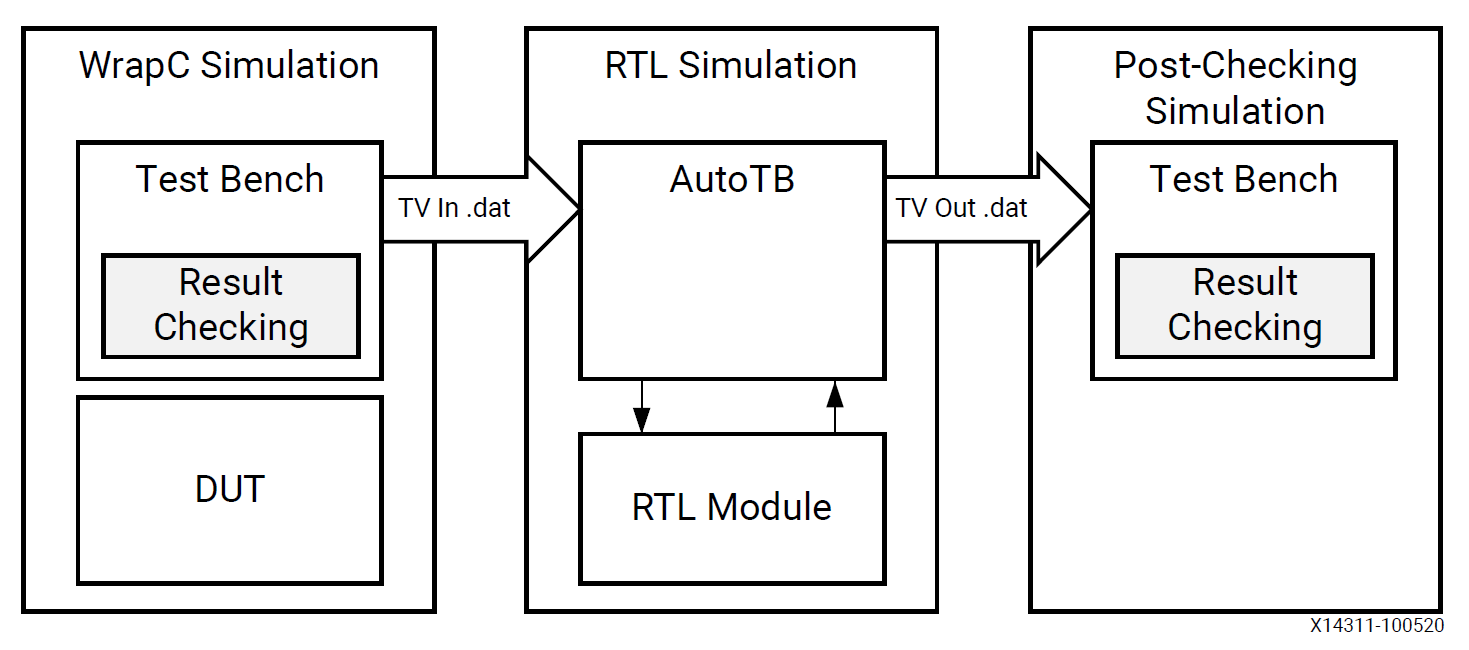
\includegraphics[width=0.9\textwidth]{images/CRTLVerification.PNG}
      \caption{C/RTL Verification Flow}
      \label{CRTLVerification.PNG}
  \end{center}
\end{figure}

C/RTL co-simulation uses a C test bench, running the main() function, to automatically verify the RTL design running in behavioral simulation. The C/RTL verification process consists of three phases:

\begin{enumerate}
  \item The C simulation is executed and the inputs to the top-level function, or the Design-Under-Test (DUT), are saved as "input vectors."
  \item The "input vectors" are used in an RTL simulation using the RTL created by Vitis HLS in Vivado simulator, or a supported third-party HDL simulator. The outputs from the RTL, or results of simulation, are saved as "output vectors."
  \item The "output vectors" from the RTL simulation are returned to the main() function of the C test bench to verify the results are correct. The C test bench performs verification of the results, in some cases by comparing to known good results.
\end{enumerate}

The following are requirements of C/RTL co-simulation:
\begin{itemize}
  \item The test bench must be self-checking as described in Writing a Test Bench, and return a value of 0 if the test passes or returns a non-zero value if the test fails.
  \item Any third-party simulators must be available in the search path to be launched by Vitis HLS.
  \item Interface Synthesis Requirements must be met (mentioned below).
  \item Any arrays or structs on the design interface cannot use the optimization directives listed in Unsupported Optimizations for Co-Simulation.
  \item IP simulation libraries must be compiled for use with third-party simulators as described in Simulating IP Cores.
\end{itemize}

Interface Synthesis Requirements: To use the C/RTL co-simulation feature to verify the RTL design, at least one of the following conditions must be true:
\begin{itemize}
  \item Top-level function must be synthesized using an ap\_ctrl\_chain or ap\_ctrl\_hs blocklevel protocol.
  \item Design must be purely combinational
  \item Top-level function must have an initiation interval of 1
  \item Interfaces must be all arrays that are streaming and implemented with axis or ap\_hs interface modes
\end{itemize}

\subsubsection{Verification of DATAFLOW and DEPENDENCE}
C/RTL co-simulation automatically verifies aspects of the DATAFLOW and DEPENDENCE directives. If the DATAFLOW directive is used to pipeline tasks, it inserts channels between the tasks to facilitate the flow of data between them. It is typical for the channels to be implemented with
FIFOs and the FIFO depth specified using the STREAM directive.

\par If co-simulation is attempted from the Vitis HLS IDE and the simulation results in a deadlock, the Vitis HLS IDE will automatically launch the Dataflow Viewer and show the processes involved in the deadlock (displayed in red). It will also show which channels are full (in red) versus empty (in white). 

\par In a similar manner, the RTL test bench is also configured to automatically check the validity of false dependencies specified using the DEPENDENCE directive. A warning message during cosimulation indicates the dependency is not false, and the corresponding directive must be removed to achieve a functionally valid design.

\subsubsection{Unsupported Optimizations for Co-Simulation}

For Vivado IP mode, automatic RTL verification does not support cases where multiple transformations are performed on arrays on the interface, or arrays within structs. In order for automatic verification to be performed, arrays on the function interface, or array inside structs on the function interface, can use any of the following optimizations, but not two or more:
\begin{itemize}
  \item Vertical mapping on arrays of the same size
  \item Reshape
  \item Partition, for dimension 1 of the array
\end{itemize}

Automatic RTL verification does not support any of the following optimizations used on a top-level function interface:
\begin{itemize}
  \item Horizontal mapping.
  \item Vertical mapping of arrays of different sizes.
  \item Conditional access on the AXI4-Stream with register slice enabled.
  \item Mapping arrays to streams.
\end{itemize}

\subsection{Analyzing RTL Simulations}
When the C/RTL co-simulation completes, the simulation report opens and  shows the measured latency and II. These results may differ from values reported after HLS synthesis. The results provided after C/RTL co-simulation show the actual values of latency and II for the given simulation data set (and may change if different input stimuli is used).

\par In non-pipelined designs, C/RTL co-simulation measures latency between ap\_start and ap\_done signals. The II is 1 more than the latency, because the design reads new inputs 1 cycle after all operations are complete.

\par In pipelined designs, the design might read new inputs before the first transaction completes, and there might be multiple ap\_start and ap\_ready signals before a transaction completes. In this case, C/RTL co-simulation measures the latency as the number of cycles between data input values and data output values. The II is the number of cycles between ap\_ready signals, which the design uses to requests new inputs.

\subsection{Cosim Deadlock Viewer}
A deadlock is a situation in which processes inside a DATAFLOW region share the same channels, effectively preventing each other from writing or reading from it, resulting in both processes getting stuck. This scenario is common when there are either FIFO's or a mix of PIPOs and FIFOs as channels inside the DATAFLOW.

\par The deadlock viewer visualizes this deadlock scenario on the static dataflow viewer. It highlights the problematic processes and channels. The viewer also provides a cross-probing capability to link between the problematic dataflow channels and the associated source code. The viewer automatically opens only after, the co-simulation detects the deadlock situation and the co-sim run has finished.

\subsection{Debugging C/RTL Co-Simulation}
When C/RTL co-simulation completes, Vitis HLS typically indicates that the simulations passed and the functionality of the RTL design matches the initial C code. 

\par Following are the primary reasons for a C/RTL co-simulation failure:
\begin{itemize}
  \item Incorrect environment setup
  \item Unsupported or incorrectly applied optimization directives
  \item Issues with the C test bench or the C source code
\end{itemize}

\section{Exporting the RTL Design}
The final step in the Vitis HLS flow is to export the RTL design in a form that can be used by other tools in the Xilinx design flow. When Vitis HLS reports the results of the high-level synthesis, it only provides an estimate of the results with projected clock frequencies and resource utilization (LUTs, DSPs, BRAMs, etc.). These results are only estimates because Vitis HLS cannot know what optimizations or routing delays will be in the final synthesized or implemented design. To get a better view of the RTL design, you can actually run Vivado synthesis and place and route on the generated RTL design, and review actual results of timing and resource utilization.

\clearpage
\section{Vitis HLS Command Line Interface}
Vitis HLS can be run from the GUI, interactively from the command line, or in batch mode from a Tcl script.

\subsection{Running Vitis HLS Interactively}
You can launch Vitis HLS using the -i option to open the tool in interactive mode.

\begin{lstlisting}[style=CStyle] 
  vitis_hls -i  // Launch Vitis HLS in interactive mode

  // The tool then displays a command line prompt
  vitis_hls> help // get a list of commands & Help for any command 

  // Vitis HLS supports an auto-complete feature by pressing the tab key
  exit // exit Vitis HLS.
  quit // quit Vitis HLS.
\end{lstlisting}

\subsection{Running Vitis HLS in Batch Mode}
Vitis HLS can also be run in batch mode, by specifying a Tcl script for the tool to run.

\begin{lstlisting}[style=CStyle]
  vitis_hls -f tcl_script.tcl  // Commands embedded in the specified 
  // script are executed in the specified sequence
\end{lstlisting}

If the Tcl script includes the exit or quit command, then the tool exits at that point, completing the batch process. If the Tcl script does not end with the exit command, Vitis HLS returns to the command prompt, letting you continue in interactive mode. All of the Tcl commands used when creating a project in the GUI are written to the solution/ script.tcl file within the project. You can use this script as a starting point for developing your own batch scripts. An example script is provided below:

\begin{lstlisting}[style=CStyle] 
  open_project dct
  set_top dct
  add_files ../dct_src/dct.cpp
  add_files -tb ../dct_src/out.golden.dat -cflags "-Wno-unknown-pragmas" -
  csimflags "-Wno-unknown-pragmas"
  add_files -tb ../dct_src/in.dat -cflags "-Wno-unknown-pragmas" -csimflags "-Wno-unknown-pragmas"
  add_files -tb ../dct_src/dct_test.cpp -cflags "-Wno-unknown-pragmas" -
  csimflags "-Wno-unknown-pragmas"
  open_solution "solution1" -flow_target vitis
  set_part {xcvu11p-flga2577-1-e}
  create_clock -period 10 -name default
  source "./dct/solution1/directives.tcl"
  csim_design
  csynth_design
  cosim_design
  export_design -format ip_catalog
\end{lstlisting}





% Chapter II Vitis HLS Hardware Design Methodology





\section{Designing Efficient Kernels}


\begin{highlight}
  Revisit  
\end{highlight}




\clearpage
\section{Vitis HLS Coding Styles}


This chapter explains how various constructs of C and C++11/C++14 are synthesized into an FPGA hardware implementation, and discusses any restrictions with regard to standard C coding.

The coding examples in this guide are available on GitHub for use with the Vitis HLS release. You can clone the examples repository from GitHub by clicking the Clone Examples command from the Vitis HLS Welcome screen.
Note: To view the Welcome screen at any time, select Help → Welcome.

\subsection{Unsupported C/C++ Constructs}
While Vitis HLS supports a wide range of the C/C++ languages, some constructs are not synthesizable, or can result in errors further down the design flow. To be synthesized:

\begin{itemize}
  \item The function must contain the entire functionality of the design.
  \item None of the functionality can be performed by system calls to the operating system.
  \item The C/C++ constructs must be of a fixed or bounded size.
  \item The implementation of those constructs must be unambiguous.
\end{itemize}

\subsubsection{System Calls}
System calls cannot be synthesized because they are actions that relate to performing some task upon the operating system in which the C/C++ program is running. Vitis HLS ignores commonly-used system calls that display only data and that have no impact on the execution of the algorithm, such as printf() and fprintf(stdout,). In general, calls to
the system cannot be synthesized and should be removed from the function before synthesis. Other examples of such calls are getc(), time(), sleep(), all of which make calls to the operating system.


\par Vitis HLS defines the macro \_\_SYNTHESIS\_\_ when synthesis is performed. This allows the \_\_SYNTHESIS\_\_ macro to exclude non-synthesizable code from the design.

\begin{highlight}
  Only the \_\_SYNTHESIS\_\_ macro should be used in the code to be synthesized. Macro in the test bench should not be used, as it is not obeyed by C/C++ simulation or C/C++ RTL co-simulation.
\end{highlight}

The \_\_SYNTHESIS\_\_ macro must not be defined or undefined in code or with compiler options, otherwise compilation might fail. The \_\_SYNTHESIS\_\_ macro is a convenient way to exclude non-synthesizable code without removing the code itself from the function, it can
result in different results between C/C++ simulation and C/C++ synthesis.

\subsubsection{Dynamic Memory Usage}
Any system calls that manage memory allocation within the system, for example, malloc(), alloc(), and free(), are not supported byt synthesis. Memory allocation system calls must be removed from the design code before synthesis. Xilinx recommends that you perform the following steps:

\begin{enumerate}[label=Step \arabic*:]
  \item Add the user-defined macro NO\_SYNTH to the code and modify the code.
  \item Enable macro NO\_SYNTH, execute the C/C++ simulation, and save the results.
  \item Disable the macro NO\_SYNTH, and execute the C/C++ simulation to verify that the results are identical.
  \item Perform synthesis with the user-defined macro disabled.
\end{enumerate}

This methodology ensures that the updated code is validated with C/C++ simulation and that the identical code is then synthesized.

\subsubsection{Pointer Limitations}
\begin{itemize}
  \item General Pointer Casting: Vitis HLS does not support general pointer casting, but supports pointer casting between native C/C++ types.
  \item Pointer Arrays: Vitis HLS supports pointer arrays for synthesis, provided that each pointer points to a scalar or an array of scalars. Arrays of pointers cannot point to additional pointers.
  \item Function Pointers: Function pointers are not supported.
  \item Pointer to pointer is not supported.
\end{itemize}

\subsubsection{Recursive Functions}
\begin{itemize}
  \item Recursive functions cannot be synthesized. This applies to functions that can form endless recursion.
  \item Vitis HLS also does not support tail recursion, in which there is a finite number of function calls.
  \item Virtual Functions are not supported.
\end{itemize}

\paragraph{Standard Template Libraries}
Many of the C++ Standard Template Libraries (STLs) contain function recursion and use dynamic memory allocation. For this reason, the STLs cannot be synthesized by Vitis HLS. The solution for STLs is to create a local function with identical functionality that does not feature recursion, dynamic memory allocation, or the dynamic creation and destruction of objects.

\subsection{Functions}
The top-level function becomes the top level of the RTL design after synthesis. Sub-functions are synthesized into blocks in the RTL design.

\begin{highlight}
  The top-level function cannot be a static function.
\end{highlight}

\subsubsection{Inlining Functions}
Sub-functions can optionally be inlined to merge their logic with the logic of the surrounding function. While inlining functions can result in better optimizations, it can also increase runtime as more logic must be kept in memory and analyzed.

\begin{highlight}
  Vitis HLS can perform automatic inlining of small functions.
\end{highlight} 

If a function is inlined, there is no report or separate RTL file for that function. The logic and loops of the sub-function are merged with the higher-level function in the hierarchy.

\subsubsection{C/C++ Builtin Functions}
Vitis HLS supports the following C/C++ builtin functions:
\begin{itemize}
  \item \_\_builtin\_clz(unsigned int x): Returns the number of leading 0-bits in x, starting at the most significant bit position. If x is 0, the result is undefined.
  \item \_\_builtin\_ctz(unsigned int x): Returns the number of trailing 0-bits in x, starting at the least significant bit position. If x is 0, the result is undefined.
\end{itemize}

\subsection{Loops}
Loops provide a very intuitive and concise way of capturing the behavior of an algorithm and are used often in C/C++ code. Loops are very well supported by synthesis. Loops can be pipelined, unrolled, partially unrolled, merged, and flattened.

\par The optimizations unroll, partially unroll, flatten, and merge effectively make changes to the loop structure as if the code were changed. These optimizations ensure that limited coding changes are required while optimizing the loops.

\begin{highlight}
  Avoid use of global variables for loop index variables, as this can inhibit some optimizations.
\end{highlight} 

The loop implementation techniques are as follows:
\begin{enumerate}
  \item Rolled implementation / iterative execution
  \item Full loop unroll
  \item Partial loop unroll
  \item Loop pipelining
\end{enumerate}

\subsubsection{Rolled implementation}
Rolled implementation or iterative execution is a default implementation. In rolled implementation, every iteration will execute in a serial and iterative manner. The loop will execute in 'n*k' cycles, where 'n' is number of loop iterations and 'k' is number of cycles required for each iteration. 
\begin{itemize}
  \item This type of implementation takes maximum time and minimum resources.
  \item The loops imply latency. Incrementing a loop counter always consumes at least one clock cycle.
  \item These rolled loops are treated as a single entity; all operations in the loop are implemented using the same hardware resources for each iteration of the loop.
\end{itemize}

\subsubsection{Full loop unroll}
In full loop unroll implementation, all the loops are removed by rewriting the operations of iterations of the loop. Loop becomes a basic block and schedule normally. This can be achieved using the following assumption:
\begin{highlight}
  There should not be any inter-iteration dependency, only then a full loop unroll can be achieved.
\end{highlight}

\begin{itemize}
  \item If a loop is completely unrolled, all operations will be performed in  parallel if data dependencies and resources allow. 
  \item In the fully unrolled version all loop operations can be performed in a single clock cycle.
  \item This type of implementation takes minimum time and maximum resources.
  \item Loops can be unrolled if their indices are statically determinable at elaboration time. They cannot be unrolled when the number of iterations is variable.
\end{itemize}

Syntax: \#pragma HLS UNROLL

\subsubsection{Partial loop unroll}
Partial loop unroll implementation is a tradeoff between Rolled implementation \& Full loop unroll implementation. In this implementation, the loop is unrolled by a certain factor provided by the designer.

\begin{highlight}
  As the loop is unrolled partially by a certain factor, the accesses/fetches from a memory are increased by the same factor. Hence, the array or memory must be split or partitioned.
\end{highlight}

Syntax: \#pragma HLS UNROLL factor=8

\begin{figure}[H]
	\begin{center}
		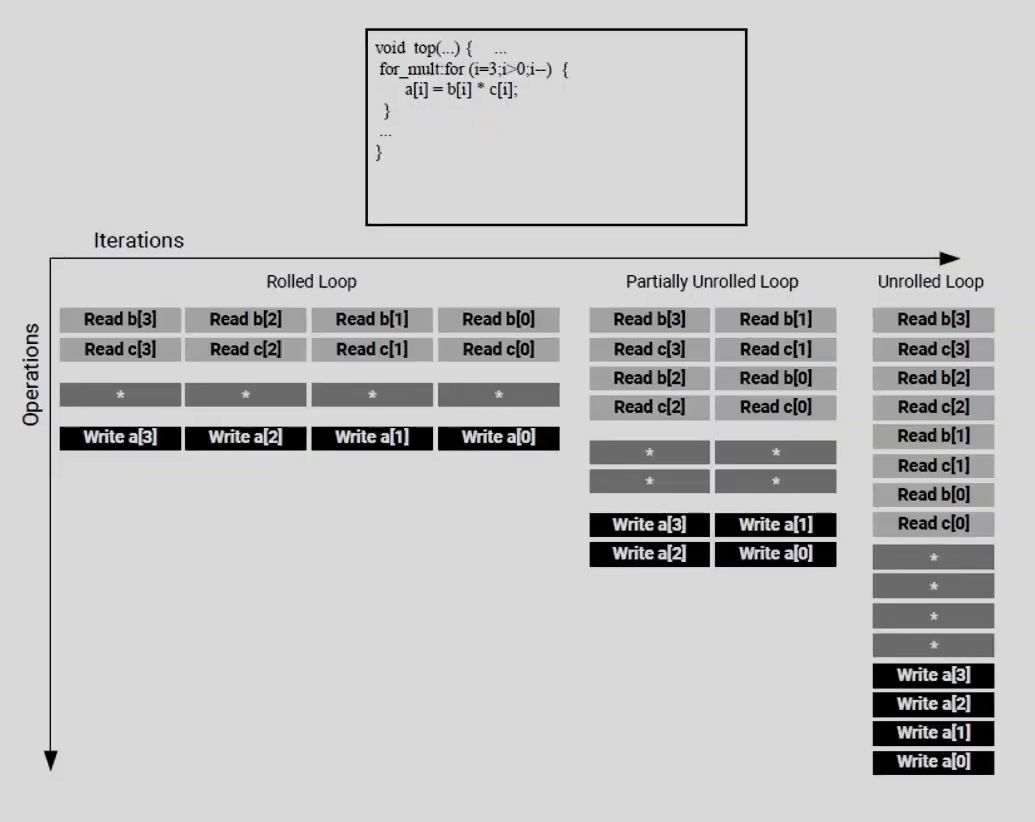
\includegraphics[width=\textwidth]{images/LoopRoll.png}
		\caption{Loop roll, unroll and partially unroll}
		\label{LoopRoll}
	\end{center}
\end{figure}

\subsubsection{Loop Pipelining}
Loop pipelining implementation allows the operations in a loop to be implemented in an overlapping manner. The pipeline executes until all iterations of the loop are completed.

\begin{figure}[H]
	\begin{center}
		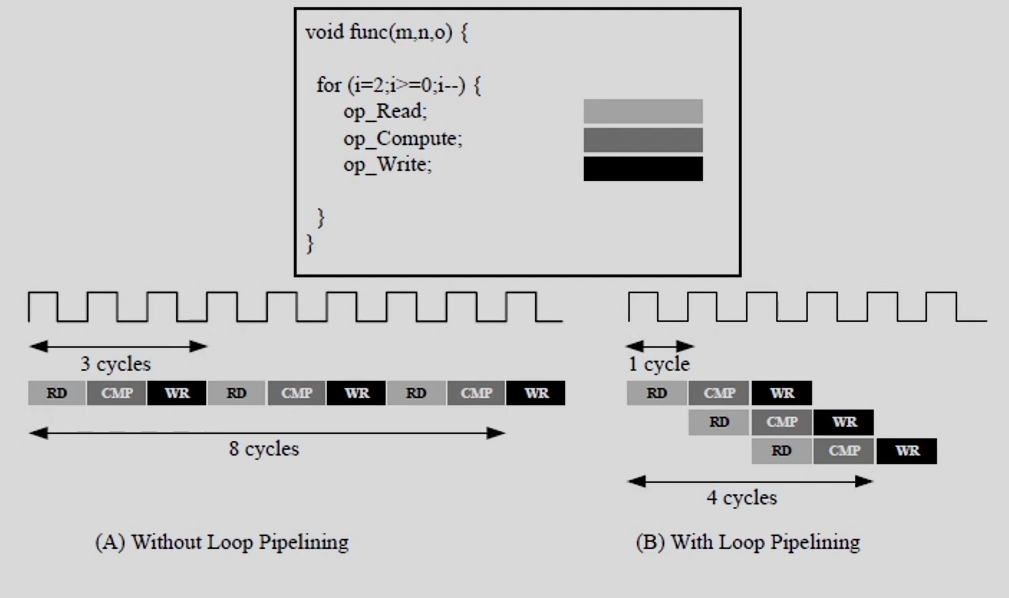
\includegraphics[width=\textwidth]{images/LoopPipe.png}
		\caption{Loop pipelining}
		\label{LoopPipe}
	\end{center}
\end{figure}

Syntax: \#pragma HLS PIPELINE II=1

\subsubsection{Nested Loop}
Having nested loops in C code is very common. In the case of nested loops:
\begin{itemize}
  \item Additional clock cycles are required to move between the rolled nested loops.
  \item One clock cycle is required to move from an outer loop to an inner loop and vice versa.
  \item When pipelining loops, the optimal balance between area and performance is typically found by pipelining the innermost loop. This also results in the fastest runtime.
  \item Pipelining the innermost loop gives the smallest hardware with generally acceptable throughput for most applications.
  \item When a loop or function is pipelined, any loop in the hierarchy below the loop or function being pipelined must be unrolled.
  \item There are three cases that can be explored: 
  \begin{enumerate}
    \item Pipelining the innermost loop (Minimum area, Good performance)
    \item Pipelining the outer loop and Unrolling the inner loop  (Low area, Better performance)
    \item Pipelining the function (Maximum area, Maximum performance)
  \end{enumerate}
\end{itemize}

The nested loops present in the code can be perfect, semi-perfect, or imperfect loops.
\begin{description}
  \item[Perfect Loops] In a perfect loop, only the innermost loop has the loop body content. There is no logic specified between the loop statements. All the loop bounds are constant.
  \item[Semi-Perfect Loops] In a semi-perfect loop, only the innermost loop has the loop body content. There is no logic specified between the loop statements. The outermost loop bound can be a variable.
  \item[Imperfect Loops] For imperfect loop nests where the inner loop has variable bounds or the loop body is not exclusively inside the inner loop, designers should try to restructure the code or unroll the loops in the loop body to create a perfect loop nest. The trivial transformation from an imperfect to perfect loop (initialization and
  final write) is made automatically by the tool. When the inner loop of a loop hierarchy is pipelined, Vitis HLS flattens the nested loops to reduce latency and improve overall throughput by removing any cycles caused by loop transitioning.
\end{description}

\subsubsection{Loop flattening}
The Vitis HLS tool provides the FLATTEN directive to allow the nested loops to be flattened, removing the need to recode for optimal hardware performance and reducing the number of cycles it takes to perform the operations in the loop.

\par The Vitis HLS tool can automatically flatten the nested loops. The recommendation is that the flattening should be specified on the innermost loop. The off option can prevent loops in the hierarchy from being flattened.

\subsubsection{Loop Merging}
Merging the loops allow the logic within the loops to be optimized together. It allows for more efficient architecture explorations.

All rolled loops imply and create at least one state in the design FSM. When there are multiple sequential loops, it can create additional unnecessary clock cycles and prevent further optimizations. The Vitis HLS tool provides the LOOP\_MERGE optimization directive, which can be
used to automatically merge the loops. The LOOP\_MERGE directive will seek to merge all the loops within the scope it is placed.


\paragraph{Loop Merging Rules}

Currently, the loop merging in the Vitis HLS tool has a few restrictions.
\begin{itemize}
  \item If loop bounds are all variables, they must have the same value.
  \item If loops bounds are constants, the maximum constant value is used as the bound of the merged loop.
  \item Loops with both variable bound and constant bound cannot be merged.
  \item Code between loops to be merged cannot have side effects: multiple execution of this code should generate the same results.
  \item Loops cannot be merged when they contain FIFO accesses. Merging would change the order of the reads and writes from a FIFO, which will affect the functioning of the FIFO.
  \item These loops can be merged using the force option.
\end{itemize}

\subsubsection{Variable Loop Bounds}
Some of the optimizations that Vitis HLS can apply are prevented when the loop has variable bounds. In this case, Vitis HLS cannot know when the loop will complete. Issues created by variable loop bounds are:

\begin{itemize}
  \item Variable loop bounds prevent Vitis HLS from determining the latency of the loop as Vitis HLS cannot statically determine the exact value of variable width, and hence, does not know the number of cycles to completely execute every iteration of the loop. Hence, variable bound loops cannot be unrolled.
  \item Another issue with variable loop bounds is that the performance of the design is unknown. There are two ways to overcome this issue: \begin{itemize}
    \item Use the pragma HLS loop\_tripcount or set\_directive\_loop\_tripcount. The tripcount is the number of loop iterations. The tripcount directive allows a minimum and/or maximum tripcount to be specified for the loop. 
    \item Use an assert macro in the C/C++ code.
  \end{itemize}  
\end{itemize}

The solution to loops with variable bounds is to make the number of loop iteration a fixed value with conditional executions inside the loop. \eg

\begin{lstlisting}[style=CStyle]
    #define N 32
    LOOP_X:for (x=0; x<N; x++) {
    if (x<width) {
    out_accum += A[x];
    }
    }
\end{lstlisting}

\subsubsection{Loop Parallelism}
Loop Parallelism refers to executing multiple loops parallely on the FPGA. Vitis HLS schedules logic and functions early as possible to reduce latency while keeping the estimated clock period below the user-specified period. To perform this, it schedules as many logic operations and functions as possible in parallel. 

\begin{itemize}
  \item Vitis HLS does not schedule loops to execute in parallel.
  \item If the loops have different bounds with same functionality, they cannot be merged. But, by placing the loops in separate functions, the identical functionality can be achieved and both loops can be scheduled in parallel as well.
  \item The principle of capturing loops in functions to exploit parallelism is presented here for cases in which dataflow optimization cannot be used.
  \item The dataflow optimization could also be used in the sequential loops.
\end{itemize}

\subsubsection{Loop Dependencies}
Loop dependencies are data dependencies that prevent optimization of loops, typically pipelining. They can be within a single iteration of a loop and or between different iteration of a loop. Loop dependencies can occur with any and all types of data. They are particularly common when
using arrays.

\subsection{Arrays}
\begin{itemize}
  \item Array is a contiguous memory. 
  \item Arrays are usually implemented as memory \ie RAM, ROM , or Registers. 
  \item Arrays on the top-level function interface are synthesized as RTL ports that access a memory outside.
  \item Internal to the design, arrays sized less than 1024 will be synthesized as FIFO. Arrays sized greater than 1024 will be synthesized into block RAM, LUTRAM, and UltraRAM depending on the optimization settings.
  \item Array access may create a bottleneck to performance. 
  \item These memories are accessed through ports. There are only a fixed number of ports(typically one or two)
\end{itemize}

\subsubsection{Minimize the parallel array access}
To mitigate this bottleneck, the designer has to minimize the parallel array access. It can be done in two ways: 
\begin{enumerate}
  \item Rewriting code to reduce memory access.
  \item Using HLS tool features to reduce the number of arrays.
\end{enumerate}

\paragraph{Rewriting code to reduce memory access}
\begin{itemize}
  \item Read array in minimum time
  \item Store locally and reuse
  \item Reduce memory access as much as possible 
\end{itemize}

\subsubsection{Array merging}
\begin{itemize}
  \item For multiple small arrays, there will be wastage of memory if we map each array to a RAM. 
  \item Small arrays can be merged into single block RAM.
  \item These small arrays should preferably have non-overlapping access.
  \item Merging can be done either horizontally or vertically. Extra locations in the memory will be padded with zeros.
  \item Syntax: \eg \#pragma HLS ARRAY\_MAP variable instance horizontal/vertical
\end{itemize}


\subsubsection{Array partitioning}
\begin{itemize}
  \item An array to be used will be larger than standard RAM size or it has many accesses.
  \item An array can be partitioned into multiple smaller arrays if it has non-overlapping accesses.
  \item Syntax: \eg \#pragma HLS array\_partition variable=<name> <type> factor=<int> dim=<int>
  
  \begin{itemize}
    \item Partition types: \begin{enumerate}
      \item Cyclic: cyclic partitioning creates smaller arrays by interleaving elements from the original array. 
      \item Block: block partitioning creates smaller arrays from blocks of the original array. This effectively splits the array into N equal blocks.
      \item Complete: complete partitioning decomposes the array into individual elements.
    \end{enumerate}
    \item factor: specifies the number of smaller arrays that are to be created.
    \item dim: specifies which dimension of a multi-dimensional array to partition.
  \end{itemize}
  \item Advantages of array partitioning: 
  \begin{itemize}
    \item Results in RTL with multiple small memories instead of one large memory.
    \item Effectively increases the amount of read and write ports for storage.
    \item Potentially improves the throughput of the design.
  \end{itemize}
\end{itemize}

\begin{figure}[H]
	\begin{center}
		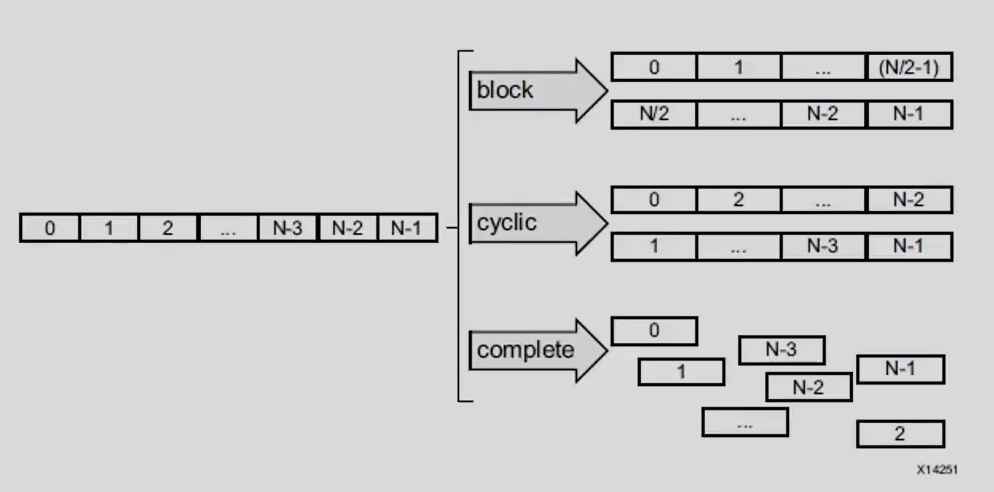
\includegraphics[width=\textwidth]{images/ArrayPart.png}
		\caption{Array partitioning}
		\label{ArrayPart}
	\end{center}
\end{figure}

\section{Defining Interfaces}
\section{Optimization Techniques in Vitis HLS}



